\begin{frame}
	\begin{block} <1-> {Eigenschaften}
		\begin{itemize}
			\item <2-> Programmiersprache: Python
			\item <3-> Umsetzung mit Heap (Priority Queue)
			\item <4-> keine Speicherung der Farbstufen wie bei Dijkstra
				\begin{itemize}
					\item <5-> kürzerer und übersichtlicherer Code
				\end{itemize}
		\end{itemize}
	\end{block}	
\end{frame}


\begin{frame}
\frametitle{Kompletter Code}
	\centering
	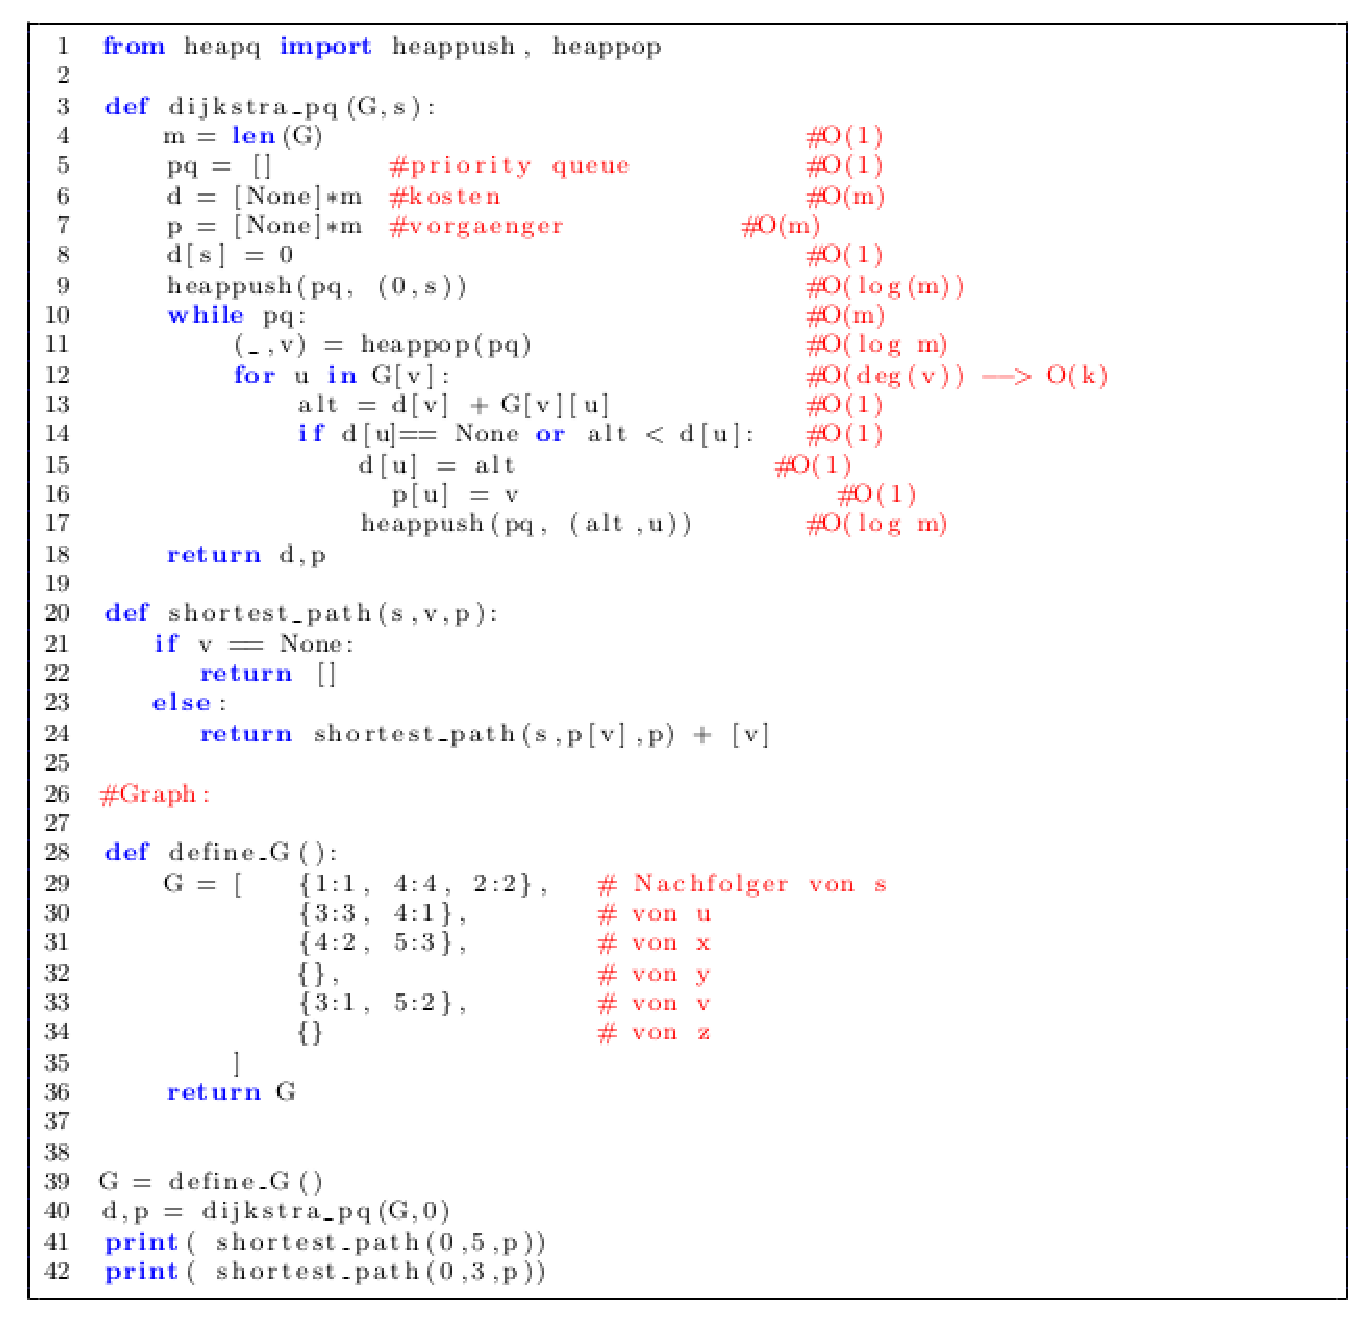
\includegraphics[scale=0.3]{./pictures/dikstra_pythonCode.eps}
\end{frame}


\begin{frame}
	\begin{block} <1-> {Eingabe}
		\begin{itemize}
			\item leer
		\end{itemize}
	\end{block}	
\end{frame}


\begin{frame}
	\begin{block} <1-> {Algorithmus}
		\begin{itemize}
		\item <1-> Initialisierung
		\item <2-> Erweitern
		\item <3-> Aktualisieren
		\end{itemize}
	\end{block}	
\end{frame}


\begin{frame}
	\begin{block} <1-> {Rekursives Bestimmen des Pfades}
		\begin{itemize}
			\item leer
		\end{itemize}
	\end{block}	
\end{frame}


\begin{frame}
	\begin{block} <1-> {Aufruf}
		\begin{itemize}
			\item leer
		\end{itemize}
	\end{block}	
\end{frame}


			

